\documentclass[12pt, a4paper]{article}
\usepackage{graphicx}
\graphicspath{ {./images/} }
%Tarih Ekleme
\usepackage[ddmmyyyy]{datetime}
\renewcommand{\dateseparator}{.}
\renewcommand{\figurename}{Şekil}
\renewcommand{\refname}{Kaynakça}

\title{El Geometrisi Tanıma}
\author{Şevval Koç \\ {sevval.koc@ogr.ksbu.edu.tr}}
\date{\today}

\begin{document}
	\begin{figure}[]
		\centering
		
\includegraphics{ksbu.jpeg}
	\end{figure}
	\maketitle
	\section{Özet}
El geometrisinden kişi tanıma özellikle istihbarat sistemlerinde kullanılan bir yöntemdir.Oluşturacağımız veri seti ile bu sistem ve çalışma prensipleri uygulanarak verimlilik ve doğruluk düzeyi incelenecektir. 

\section{Giriş}
Biyometrik uygulamalar için de
Yüz, el geometrisi ve iris ise son yıllarda ilginin arttığı ve
kullanılmaya başlanan özelliklerdir. Bunda özelliklerin
işlenmek üzere elde edilmesinin kolaylaşması önemli bir
etkendir.
El geometrisi tanıma Amerika’da 20.YY' dan beri kullanılan,özellikle havaalanları ve nükleer güç istasyonlarında tercih edilen bir yöntemdir.Bu metotta, kullanılan sisteme göre kişilerin elinin veya iki parmağının geometrik yapısı analiz edilir.Parmakların uzunluğu,genişliği ve büküm noktaları ayırt edici özelliklerdir.
Biyometrik tanıma sistemleri için öncelikle bir görüntü
kaydedilir. Kaydedilen bu görüntü sayısal koda çevrilir. Bu
kod da yapılan işleme göre şifrelenir ve bilgisayara kaydedilir.
Daha sonra kullanıcı herhangi bir cihaz kullanarak kendini
sisteme tanıtır. Kullanıcının kendini sisteme tanıttığı andaki
duruşu ve çevre koşullarından dolayı sistem de kayıtlı olan
sayısal kod ile doğrulama aşamasında üretilen kodun birbiriyle
tamamıyla aynı olma olasılığı yoktur. Bu sayede el geometrisine göre kişi ayırt etme güvenli bir tanıma sistemi haline gelmektedir 
\section{Yöntem}

Kişilerin el geometrilerine ait verilerinin kullanılacağı veri seti oluşturulur.Bunun için ilk aşamada veri toplama standartı belirlenir.Bu standarta göre her kişiden siyah düz bir zeminde belirli sabit bir mesafeden ellerinin iç ve dış yüzeylerini fotoğraflanır.Sonraki aşamalarda bu fotoğraflar etiketlenir. Daha sonra verilerin işlenmeye hazır hale gelebilmesi için tüm verileri ön işleme ile standart boyutlu hale kenar mesafeleri belirli ölçüde hale getirilecektir.Sıradaki adımda El geometrisi özelliklerini tanımlamak için görüntü işleme teknikleri kullanılacaktır. Bu adımda, elin konturunu (dış hat), elin dış görünümünü, parmak pozisyonlarını, parmak uzunluklarını ve genişliklerini belirlemek için algoritmalar uygulanacaktır. Sonraki adımda el geometrisi özelliklerinin çıkarımını yapmak için belirlenen el geometrisi özellikleri üzerinden özellik vektörleri çıkarılır. Bu özellik vektörleri, her bir elin benzersiz özelliklerini tanımlar. Bu adımdan sonra elde edilen vektörler, makine öğrenimi algoritmaları kullanılarak eğitilir. Bu adımda, sınıflandırma algoritmaları veya derin öğrenme modelleri gibi teknikler kullanılabilir. Eğitim veri setindeki özellik vektörleri ve ilgili sınıf etiketleri (kişilerin kimlikleri) kullanılarak bir model oluşturulur. Son olarak oluşturulan model, ayrılmış test veri seti üzerinde değerlendirilir. Modelin doğruluğu, hassasiyeti gibi performans özellikleri kullanılarak değerlendirilecektir. 

\section{Literatür araştırması}

\begin{enumerate}
	
	\item El Geometrisi Tabanlı Kimlik Doğrulama Çalışmaları:
			\begin{figure}[!h]
		\centering
		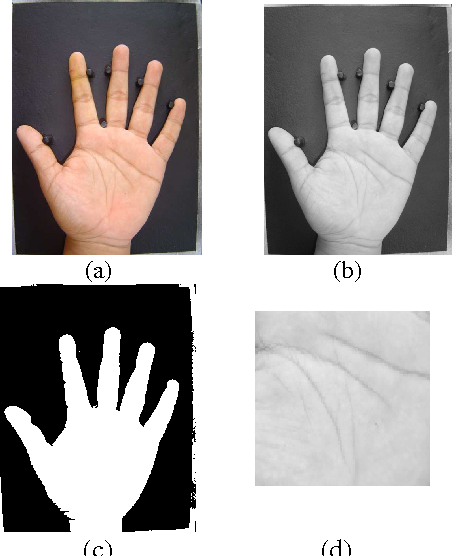
\includegraphics{hand2.png}
	\end{figure}
		
	El geometrisinin orta düzeyde güvenlik sağladığı düşünülmektedir, ancak çeşitli avantajları vardır
	diğer tekniklerle karşılaştırıldığında:
	\begin{enumerate}
		\item  Sadece bir platforma ve ortama ihtiyaç duyduğu için orta maliyetli
		çözünürlüklü okuyucu veya kamera,
		\item  düşük hesaplama maliyetli algoritma kullanır, bu da
		hızlı sonuçlar için,
		\item  düşük şablon boyutu (352'den 1209 bayta kadar)
		depolama ihtiyaçlarını azaltır,
		\item  kullanıcılar için çok kolay ve caziptir 
		
		\item  adli işlemler ve suçlu kaydı için kolaylık sağlar \cite{varchol2007using}.

	\end{enumerate}
	\cite{ergen2011biyometrik}.

	\item  Diğer bimodal biyometrik sistemlerin aksine, avuç izi ve el geometrisi özellikleri aynı anda dijital kamera kullanılarak aynı görüntüden elde edilebildiğinden, kullanıcıların iki sensörden geçme zahmetine katlanmaları gerekmez. Bu gri seviye görüntülerin her biri hizalanır ve ardından avuç izi ve el geometrisi özelliklerini çıkarmak için kullanılır. Bu özellikler daha sonra bireysel ve birleşik performansları açısından incelenir \cite{kumar2003personal}.

\end{enumerate}
	
	\bibliographystyle{plain}
\bibliographystyle{ieeetr}
\bibliography{references.bib} 	
\end{document}